\documentclass[12pt]{article}
\usepackage{amsmath, amssymb, amsthm}
\usepackage{geometry}
\usepackage{xcolor}
\usepackage{graphicx}
\usepackage{nicematrix}
\usepackage{booktabs}
\usepackage{tikz}
\geometry{margin=1in}

\title{Engineering Probability \\ Homework 5}
\author{Timothy Pollard, pollat@rpi.edu}
\date{October 5th 2025}

\begin{document}
\maketitle
\hrule



\section*{(1)} Given a random variable $X$ with mean $\mu_X$ and variance $\sigma_X^2$, 
find the mean and variance of the standardized random variable
\[
Y = \frac{1}{\sigma_X}(X - \mu_X).
\]
    \textcolor{blue}{\[\mu_Y=E[Y]=\frac{1}{\sigma_X}(E[X-\mu_X])=\frac{1}{\sigma_X}(0)=0\]}
    \textcolor{blue}{\[\sigma_Y^2=\text{Var}(Y)=\left(\frac{1}{\sigma_X}\right)^2(\text{Var(X)})=\left(\frac{1}{\sigma_X^2}\right)(\sigma_X^2)=1\]}
\newpage

\section*{(2)} The random variable $X$ has CDF
    \[
    F_X(x) =
    \begin{cases}
    0, & x < -1, \\
    0.2, & -1 \leq x < 0, \\
    0.7, & 0 \leq x < 1, \\
    1, & x \geq 1.
    \end{cases}
    \]
\begin{enumerate}
    \item[(a)] Draw a graph of the CDF.
        \begin{center}
            \includegraphics[width=0.5\textwidth]{CDF1.png}
        \end{center}
    \item[(b)] Write $P_X(x)$, the PMF of $X$. Be sure to write the value of $P_X(x)$ for all $x$ from $-\infty$ to $\infty$.
        \textcolor{blue}{\[
        P_X(x) =
        \begin{cases}
        0.2, &  x =-1, \\
        0.5, &  x = 0, \\
        0.3, & x =1,\\
        0 & \text{otherwise}. \\ 
        \end{cases}
        \]}
\end{enumerate}

\section*{(3)} A grocery store sells $X$ hundred kilograms of rice every day, where the distribution of $X$ is:
    \[
    F(x) =
    \begin{cases}
    0, & x < 0, \\
    kx^2, & 0 \leq x < 3, \\
    k(-x^2 + 12x - 3), & 3 \leq x < 6, \\
    1, & x \geq 6.
    \end{cases}
    \]

Suppose that this grocery store’s total sales of rice do not reach 600 kilograms on any given day.
\begin{enumerate}
    \item[(a)] Find the value of $k$.
        \textcolor{blue}{\[k(-(6)^2+12(6)-3)=1\]
        \[k(-36+72-3)=1\]
        \[k(33)=1 \therefore \boxed{k=\frac{1}{33}}\]}
    \item[(b)] What is the probability that the store sells between 200 and 400 kilograms of rice next Thursday?
        \textcolor{blue}{\[F_X(4)-F_X(2)=P(2<X\leq4)\]
        \[P(2<X\leq4)=\frac{1}{33}\left(-(4)^2+12(4)-3 \right) - \frac{1}{33}(2)^2\]
        \[P(2<X\leq4)=\frac{1}{33}\left(-(16)+48-3 \right) - \frac{4}{33}\]
        \[P(2<X\leq4)=\frac{1}{33}\left(29\right) - \frac{4}{33}\]
        \[P(2<X\leq4)=\frac{25}{33}\boxed{=0.75\overline{75}}\]}
    \item[(c)] What is the probability that the store sells over 300 kilograms of rice next Thursday
        \textcolor{blue}{\[P(X>3)= 1-P(X\leq3)= 1-F_X(3)\]
        \[P(X>3)=1-\frac{1}{33}\left(-(3)^2+12(3)-3\right)\]
        \[P(X>3)=1-\frac{1}{33}\left(-(9)+36-3\right)\]
        \[P(X>3)=1-\frac{1}{33}\left(24\right)\]
        \[P(X>3)=1-\frac{1}{33}\left(24\right)\]
        \[P(X>3)=\frac{9}{33}=\frac{3}{11}\boxed{=0.27\overline{27}}\]}
    \item[(d)] Given that the store sold at least 300 kilograms of rice last Friday, what is the probability that it did not sell more than 400 kilograms on that day?
        
        \textcolor{blue}{\[P(X\leq4|X\geq3)=\frac{P(X\leq4\cap X\geq3)}{P(X\geq3)}=\frac{F_X(4)-F_X(3^-1)}{1-F_X(3^-1)}\]}
        \textcolor{blue}{\[F_X(4)=\frac{1}{33}(-(4)^2+12(4)-3)=\frac{29}{33}\]}
        \textcolor{blue}{\[F_X(3^-)=\frac{1}{33}(3^2)=\frac{9}{33}\]}
        \textcolor{blue}{\[P(X\leq4|X\geq3)=\frac{\frac{29}{33}-\frac{9}{33}}{1-\frac{9}{33}}=\frac{\frac{20}{33}}{\frac{24}{33}}=\frac{5}{6}\]}
\end{enumerate}

\section*{(4)} The cumulative distribution function of random variable $X$ is
    \[
    F_X(x) =
    \begin{cases}
    0, & x < -1, \\
    \dfrac{x+1}{2}, & -1 \leq x < 1, \\
    1, & x \geq 1.
    \end{cases}
    \]
Find the PDF $f_X(x)$ of $X$.
    \textcolor{blue}{
    \[f_X(x)=\frac{dF_X(x)}{d x} \]
    \[f_X(x) =
    \begin{cases}
    0, & x < -1, \\
    \dfrac{1}{2}, & -1 \leq x < 1, \\
    0, & x \geq 1.
    \end{cases}
    \]
    }

\section*{(5)} The probability density function of random variable $X$ is
    \[
    f_X(x) =
    \begin{cases}
    \dfrac{1}{2}e^{-x/2}, & x \geq 0, \\
    0, & \text{otherwise}.
    \end{cases}
    \]

\begin{enumerate}
    \item[(a)] What is $P[1 \leq X \leq 2]$?
        \textcolor{blue}{ \[\int_{1}^{2}{f_X(x)dx}=P[1 \leq X \leq 2]\]
        \[P[1 \leq X \leq 2]=\int_{1}^{2}{\left(\frac{1}{2}e^{-\frac{x}{2}}\right)dx}\]
        \[P[1 \leq X \leq 2]=\frac{1}{2}\left. \left(-2e^{-\frac{x}{2}}\right)\right\rvert_1^2\]
        \[P[1 \leq X \leq 2]=\left. \left(-e^{-\frac{x}{2}}\right)\right\rvert_1^2\]
        \[P[1 \leq X \leq 2]=\left(-e^{-\frac{(2)}{2}}\right)-\left(-e^{-\frac{(1)}{2}}\right)\]
        \[P[1 \leq X \leq 2]=\left(-\frac{1}{e}\right)+\left(\frac{1}{e^{\frac{1}{2}}}\right) \boxed{\approx 0.239}\]
        }
    \item[(b)] What is $F_X(x)$, the cumulative distribution function of $X$?
        \textcolor{blue}{\[F_X(x)=\int_{-\infty}^{x}f_X(x)dx\]
        \[F_X(x)=\int_{0}^{x}\left(\frac{1}{2}e^{\frac{-x}{2}}\right)dx\text{ (for } x\geq 0)\] 
        \[F_X(x)=\left. \left(-e^{-\frac{x}{2}}\right)\right\rvert_0^x=\left(-e^{-\frac{x}{2}}\right)+1\]
        \[\boxed{ F_X(x) =
        \begin{cases}
        0, & x <0 \\
        -e^{-x/2}+1, & x \geq 0.
        \end{cases}
        }\]}
    \item[(c)] What is $E[X]$, the expectation of $X$?
         \textcolor{blue}{\[E[X]=\int_{0}^{\infty}{x\frac{1}{2}e^{\frac{-x}{2}}}dx=\frac{1}{2}\int_{0}^{\infty}{xe^{\frac{-x}{2}}}dx\]}
            \textcolor{blue}{
            \[
            \renewcommand{\arraystretch}{1.5}
            \begin{NiceArray}{c @{\hspace*{1.0cm}} c}[create-medium-nodes]
            \toprule
                D & I \\
            \cmidrule{1-2}
                x & e^{\frac{-x}{2}} \\
                1  & -2e^{\frac{-x}{2}} \\      
                0   & 4e^{\frac{-x}{2}} \\      
            \bottomrule
            \CodeAfter
            \begin{tikzpicture} [->, name suffix = -medium]
            \draw [blue] (2-1) -- node [above] {$+$} (3-2) ; 
            \draw [red] (3-1) -- node [above] {$-$} (4-2) ; 
            \end{tikzpicture}
            \end{NiceArray}
            \quad E[X]=\frac{1}{2}\left.\left(-2xe^{\frac{-x}{2}}-4e^{\frac{-x}{2}}\right)\right\rvert_0^{\infty}
            \]
        \[E[X]=-1\left.\left(xe^{\frac{-x}{2}}-2e^{\frac{-x}{2}}\right)\right\rvert_0^{\infty}\]
        \[E[X]=\lim_{t \to \infty}\left(-1\left(te^{\frac{-t}{2}}-2e^{\frac{-t}{2}}\right)\right)-\left((0)e^{\frac{-(0)}{2}}-2e^{\frac{-(0)}{2}}\right)\]
        \[E[X]=0-\left(-2\right)=\boxed{2}\]}
    \item[(d)] What is $\text{Var}[X]$, the variance of $X$?
        \textcolor{blue}{\[E[X^2]=\int_{0}^{\infty}{x^2\frac{1}{2}e^{\frac{-x}{2}}}dx\]}
            \textcolor{blue}{
            \[
            \renewcommand{\arraystretch}{1.5}
            \begin{NiceArray}{c @{\hspace*{1.0cm}} c}[create-medium-nodes]
            \toprule
                D & I \\
            \cmidrule{1-2}
                x^2 & e^{\frac{-x}{2}} \\
                2x  & -2e^{\frac{-x}{2}} \\      
                2   & 4e^{\frac{-x}{2}} \\     
                0   & -8e^{\frac{-x}{2}} \\
            \bottomrule
            \CodeAfter
            \begin{tikzpicture} [->, name suffix = -medium]
            \draw [blue] (2-1) -- node [above] {$+$} (3-2) ; 
            \draw [red] (3-1) -- node [above] {$-$} (4-2) ; 
            \draw [blue] (4-1) -- node [above] {$+$} (5-2) ; 
            \end{tikzpicture}
            \end{NiceArray}
            \quad E[X^2]=\frac{1}{2}\left.\left(-2x^2e^{\frac{-x}{2}}-8xe^{\frac{-x}{2}}-16e^{\frac{-x}{2}}\right)\right\rvert_0^{\infty}
            \]
        \[E[X^2]=-1e^{\frac{-x}{2}}\left.\left(x^2+4x+8\right)\right\rvert_0^{\infty}\]
        \[E[X^2]=\lim_{t \to \infty}\left(-1e^{\frac{-t}{2}}\left(t^2+4t-8\right)\right)-\left(-1e^{\frac{-(0)}{2}}\left((0)^2+4(0)+8\right)\right)\]
        \[E[X^2]=\left(0\right)-\left(-1(1)\left(-8\right)\right)=8\]
        \[\boxed{\text{Var}(X)=E[X^2]-E[X]^2=8-2^2=4}\]}
\end{enumerate}

\section*{(6)} Continuous random variable $X$ has PDF
    \[
    f_X(x) =
    \begin{cases}
    \dfrac{1}{4}, & -1 \leq x \leq 3, \\
    0, & \text{otherwise}.
    \end{cases}
    \]

Define the random variable $Y$ by $Y = h(X) = X^2$.
    \begin{enumerate}
        \item[(a)] Find $E[X]$ and $\text{Var}[X]$.
            \textcolor{blue}{\[E[X]=\frac{(3+(-1))}{2}=\boxed{1}\]
            \[\text{Var}(X)=\frac{(3-(-1))^2}{12}=\frac{16}{12}=\boxed{\frac{4}{3}}\]}
        \item[(b)] Find $h(E[X])$ and $E[h(X)]$.
            \textcolor{blue}{\[h(E[X])=h(1)=\boxed{\frac{1}{8}}\]
            \[E[h(X)]=E[X^2]=\int_{-1}^{3}{\frac{1}{4}}x^2dx=\left.\frac{1}{12}x^3\right\rvert_{-1}^3=\frac{(3)^3}{12}-\frac{(-1)^3}{12}=\frac{28}{12}=\boxed{\frac{7}{3}}\]}
        \item[(c)] Find $E[Y]$ and $\text{Var}[Y]$.
            \textcolor{blue}{\[E[Y]=E[H(X)]=\boxed{\frac{7}{3}}\]}
            \textcolor{blue}{\[E[X^4]=\int_{-1}^{3}{\frac{1}{4}x^4}=\left.\frac{1}{20}x^5\right\rvert_{-1}^3=\frac{1}{20}(3)^5-\frac{1}{20}(-1)^5=\frac{244}{20}=\frac{61}{5}\]}
            \textcolor{blue}{\[\text{Var}[Y]=E[X^4]-(E[X^2])^2=\frac{61}{5}-\left(\frac{7}{3}\right)^2=\frac{304}{45}=\boxed{6.7\overline{5}}\]}
    \end{enumerate}
\newpage 

\section*{(7)} Let $X$ be a random variable with CDF
    \[
    F_X(x) =
    \begin{cases}
    0, & x < -1, \\
    \dfrac{x}{3} + \dfrac{1}{3}, & -1 \leq x < 0, \\
    \dfrac{x}{3} + \dfrac{2}{3}, & 0 \leq x < 1, \\
    1, & x \geq 1.
    \end{cases}
    \]

Sketch the CDF and find:\\
    \begin{center}
        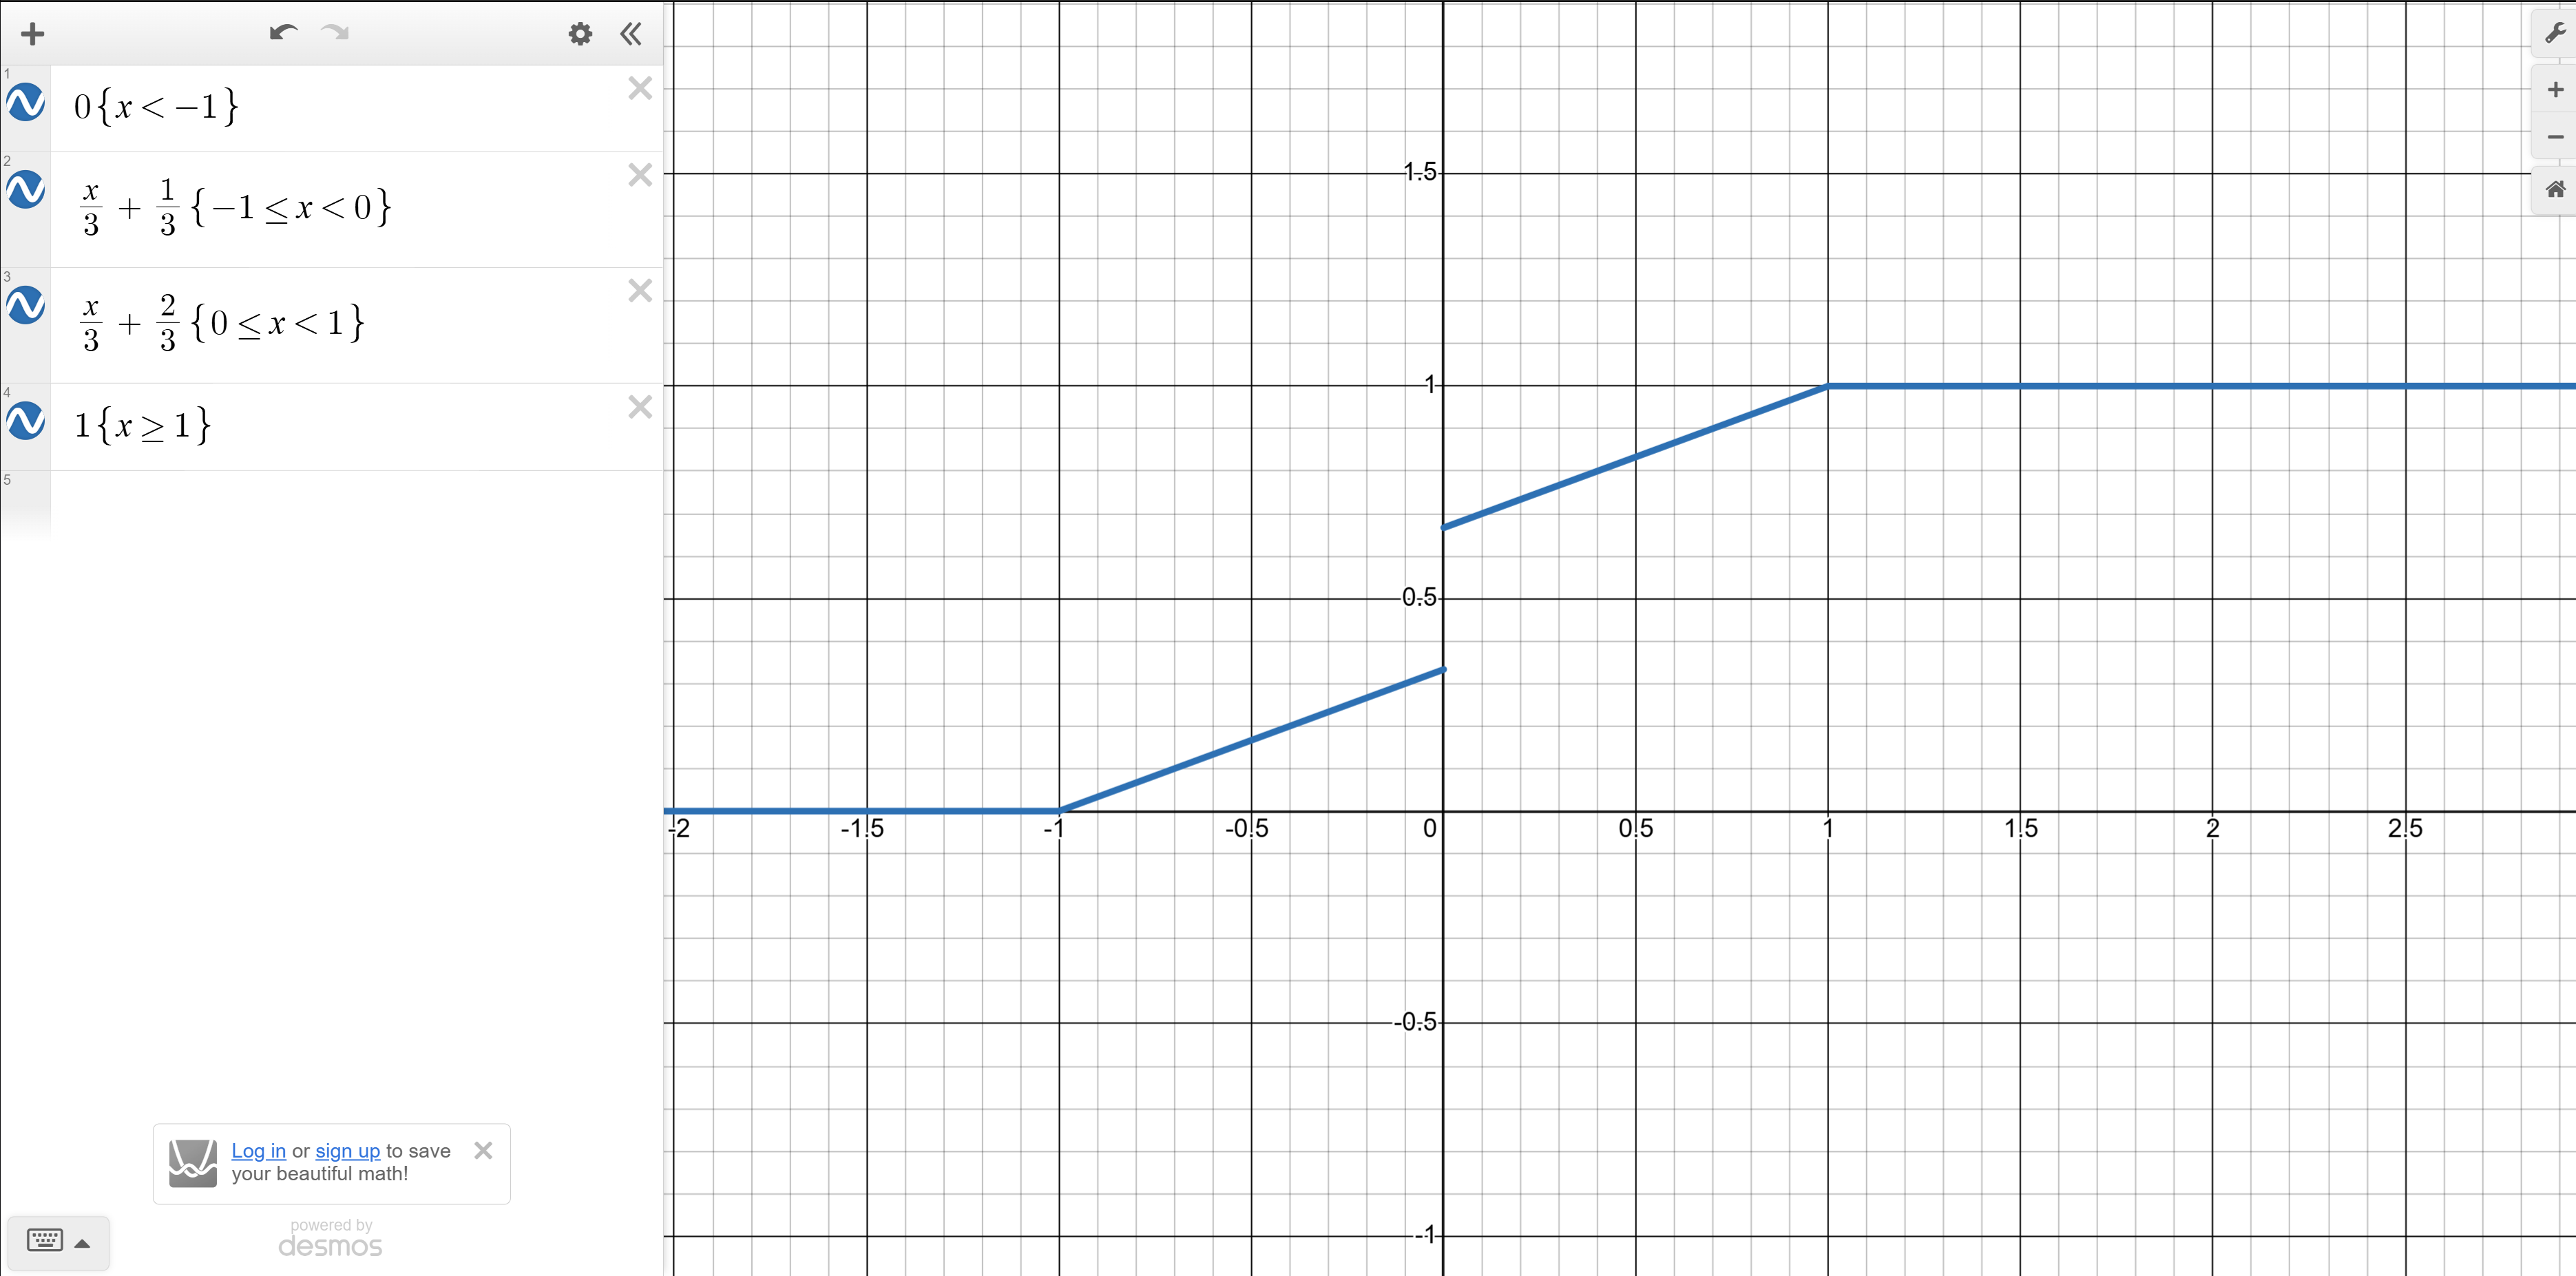
\includegraphics[width=0.75\textwidth]{CDF7.png}
    \end{center}
\begin{enumerate}
    \item[(a)] $P[X < -1]$ and $P[X \leq -1]$
        \textcolor{blue}{\[P[X<-1]=0 \qquad P[X\le -1]=F(-1)=0\]}
    \item[(b)] $P[X < 0]$ and $P[X \leq 0]$
        \textcolor{blue}{\[P[X<0]=F(0^-)=\frac{1}{3},\qquad P[X\le0]=F(0^+)=\frac{2}{3}.\]}
    \item[(c)] $P[0 < X \leq 1]$ and $P[0 \leq X \leq 1]$
        \textcolor{blue}{\[P(0<X\le1)=F(1)-F(0^+)=1-\frac{2}{3}=\frac{1}{3},
\qquad
P(0\le X\le1)=F(1)-F(0^-)=1-\frac{1}{3}=\frac{2}{3}.
\]}
    \item[(d)] $f_X(x)$
        \textcolor{blue}{\[f_X(x)=\frac{dF_X}{dx}= \frac{1}{3}\delta(x)+
\begin{cases}
0,& x<-1,\\[4pt]
\frac{1}{3},& -1\le x<0,\\[4pt]
\frac{1}{3},& 0<x<1,\\[4pt]
0,& x\ge1,
\end{cases}
\]}
    \item[(e)] $E[X]$
    \textcolor{blue}{\[E[x]=0\](PDF is symmetric about x=0)}
    \item[(f)] $\text{Var}[X]$
    \textcolor{blue}{\[
\begin{aligned}
E[X^2]&=\int_{-1}^{0}\frac{1}{3}x^2\,dx \;+\; 0^2\cdot P(X=0) \;+\;\int_{0}^{1}\frac{1}{3}x^2\,dx\\
&=\frac{1}{3}\left(\frac{x^3}{3}\Big|_{-1}^{0}\right)+\frac{1}{3}\left(\frac{x^3}{3}\Big|_{0}^{1}\right)\\
&=\frac{1}{3}\left(\frac{1}{3}\right)+\frac{1}{3}\left(\frac{1}{3}\right)=\frac{2}{9}\\
\mathrm{Var}(X)&=E[X^2]-\big(E[X]\big)^2=\frac{2}{9}-0^2=\boxed{\frac{2}{9}}
\end{aligned}
\]}
\end{enumerate}
\end{document}

